\chapter{Data}
\section{Introduction}
The PK models in this section will be fitted using NLMM with the nlmixr2 package \citep{nlmixr, nlmixrarticle}. To be able to fit a model, a model specification, a dataset, and an estimation method must be provided.

The model specification must include initial values and potential boundaries for $\beta$, residual error variance, $\sigma^2$, and for the entries in $\Omega$. The functional forms of the $p$ entries in $d$ from \eqref{eq: NLME Stage 2}, along with the error model, must be specified.
The functional form of \ref{eq: NLME Stage 1} is specified by solving a system of given ODEs describing the mass balance equations for the given compartments, e.g. \eqref{eq: first order kinetic of amount in one com without abs}, \eqref{eq: first order kinetic of amount in central com with abs com}, or \eqref{eq: 2-comp central}.

% data structure
The data require at least a unique subject identifier, timestamp of the observations, a dependent variable, an amount or rate of drug, and an event identifier to describe the observation \citep{nlmixrarticle}. 

% estimation method
The FOCEI, covered in \ref{sec: Estimation methods}, is used as the estimation method, however, other methods, e.g. FO, FOCE, and saem, are also supported. 


%output
% The output of the nlmixr function is metrics of goodness of fit, i.e. objective function, information criteria, log likelihood, and condition number, the run time of the fitting process, the subject specific parameters with standard errors, residual squared error, BSV, and shrinkage, the fitted omega matrix and lastly the fitted data 

% metrics of goodness of fit
% The run time to fit the model
% the population parameter estimates + residual error
% Omega matrix
% fitted values for $\beta$s, $\eta$s and $\e_i$s
\section{Introduction to data}

\begin{table}[h]
    \centering
    \caption{Values data is simulated from}
    \label{table:parameter_estimates}
    \resizebox{\textwidth}{!}{%
        \begin{tabular}{@{}llcccccc@{}}
            \toprule
            Parameter                                   & Estimate         & (95\% CI)              & RSE (\% CV) & IIV (\% CV) & Shrinkage (\%) \\ \midrule
            Absorption rate constant ($k_a$)           & 0.0253          & [0.0236--0.027]       & 3.42        & 37.9       & 9.4157         \\
            Clearance (CL), L/h                         & 0.0348          & [0.0327--0.0369]      & 3.06        & 15.2       & 1.5202         \\
            Central volume ($V_c$), L                   & 3.59            & [3.28--3.9]           & 4.44        & 15.4       & 6.6167         \\
            Intercompartmental clearance ($Q$), L/h     & 0.304           & [0.249--0.359]        & 9.19        & 15.2       & 1.5202         \\
            Peripheral volume ($V_p$), L                 & 4.10            & [3.78--4.42]          & 3.97        & 15.4       & 6.6167         \\ \bottomrule
        \end{tabular}%
    }
\end{table}
Data is single dose concentration profiles simulated from a two-compartment model with depot. The following is based on simulated profiles with added proportional residual error. 


In the following, nlmixr will be used to fit a two-compartment model with depot, with $\theta_i=(k_{a,i}, CL_{i}, Q_i,V_{c,i},V_{p,i})^\top$ specified in a number of ways.

All models are fitted on 10, 25, 50 and 100 sample profiles, respectively, using focei estimation, unless mentioned otherwise. 

\section{Population model}
The first model is fitted with $\theta_i=(k_{a,\mu}, CL_{\mu}, Q_{\mu},V_{c,\mu},V_{p,\mu})^\top$, i.e. without any random effects, making it a population only model. 

Figure 'DV vs. IPRED 100sp focei' shows that focei significantly underestimates the concentration, a trend also observed with 10, 25, and 50 sample profiles. Consequently, the parameter estimates from focei are far from the true values, see Figure 'Boxplot of estimated differences'. Estimation with non-linear least squares (nls) captures the population trend, as shown in Figure 'DV vs. IPRED 100sp nls'. The spread of observations around the population prediction suggests that allowing for individual variability could be beneficial. The concentration profiles along with the estimated population estimate is shown in Figures 'DV vs. IPRED 10sp' and 'DV vs. IPRED 100sp' for 10 and 100 concentration profiles, respectively.

The estimated residual standard deviation is, for 10, 25, 50, 100 sample profiles; 0.1901, 0.2555, 0.2768, 0.2781. The more sample profiles the model is fitted on, the more accurate parameter estimates and lower standard errors, see Figure 'estimated differences'.

\begin{table}
\centering\centering
\caption{NLS No BSV - DV 100}
\centering
\fontsize{8}{10}\selectfont
\begin{tabular}[t]{lllllll}
\toprule
\textbf{Parameter} & \textbf{Est} & \textbf{SE} & \textbf{\%RSE} & \textbf{Back-transformed} & \textbf{BSV} & \textbf{Shrinkage}\\
\midrule
tka & -3.491 & 0.7265 & 20.81 & 0.03047 (0.007337, 0.1266) &  & \\
\midrule
tq & -0.6653 & 4.159 & 625 & 0.5141 (0.0001483, 1782) &  & \\
\midrule
tcl & -3.47 & 0.06542 & 1.885 & 0.03112 (0.02738, 0.03538) &  & \\
\midrule
tvc & 1.212 & 1.224 & 101 & 3.36 (0.3054, 36.96) &  & \\
\midrule
tvp & 1.379 & 1.084 & 78.59 & 3.971 (0.4747, 33.22) &  & \\
\midrule
prop.sd & 0.2781 &  &  & 0.2781 &  & \\
\bottomrule
\end{tabular}
\end{table}

\begin{figure}[htbp]
    \centering
    % First 2x2 grid
    \begin{subfigure}[b]{0.49\linewidth}
        \centering
        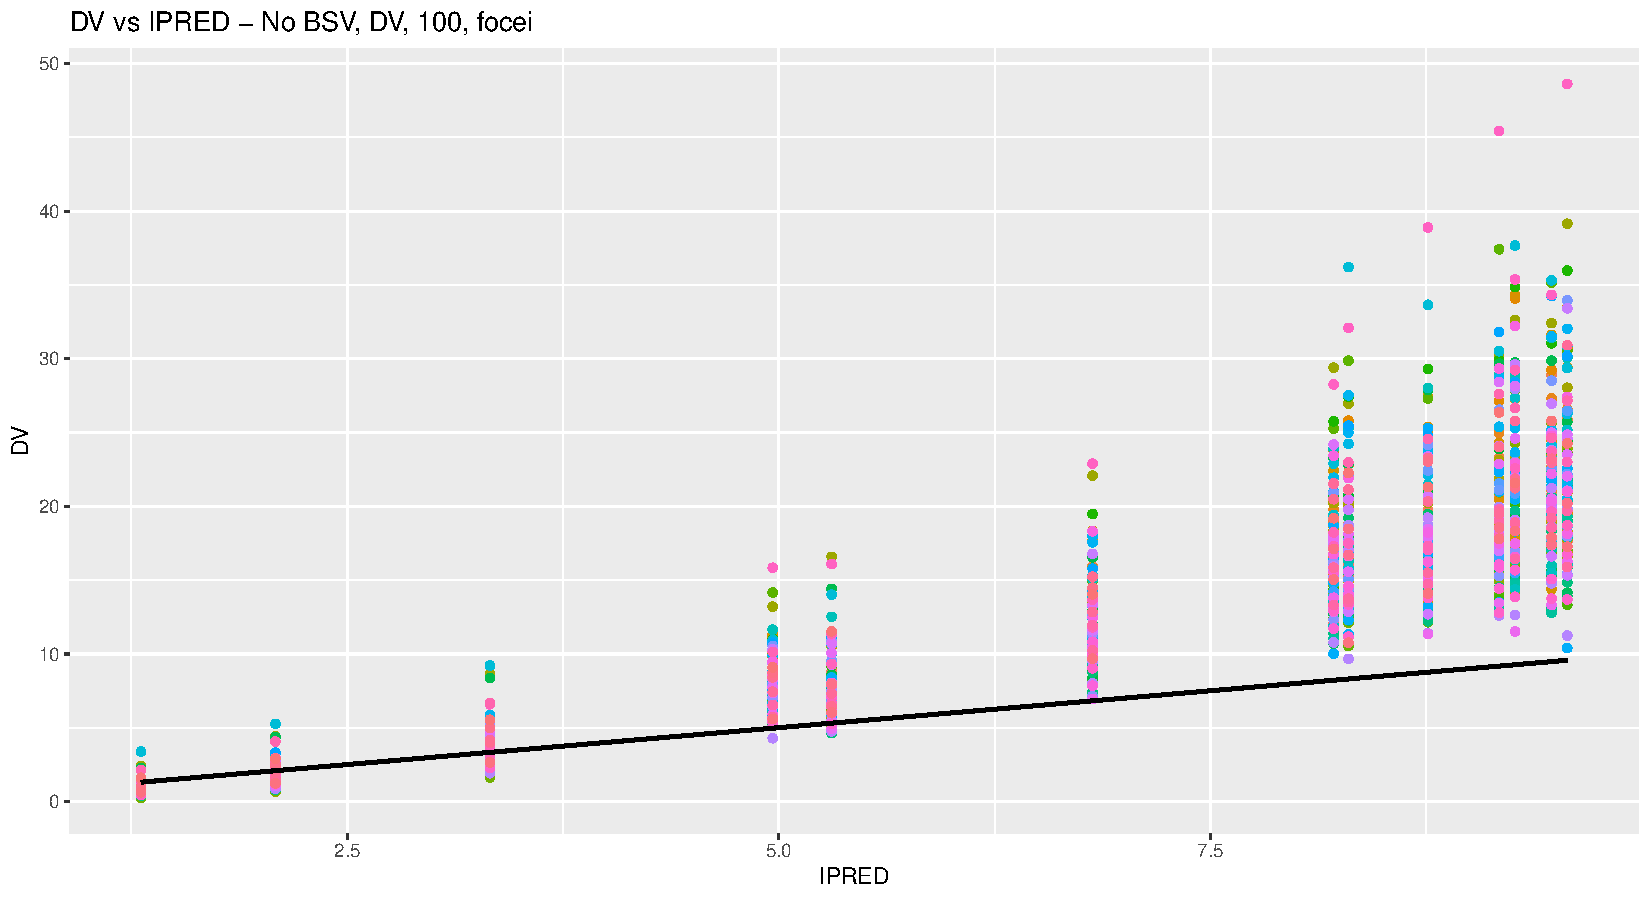
\includegraphics[width=\linewidth]{fig/img/Xpose/nobsv/dv_vs_ipred_100_focei_plot.pdf}
        \caption{}
        \label{fig:}
    \end{subfigure}
    \hfill
    \begin{subfigure}[b]{0.49\linewidth}
        \centering
        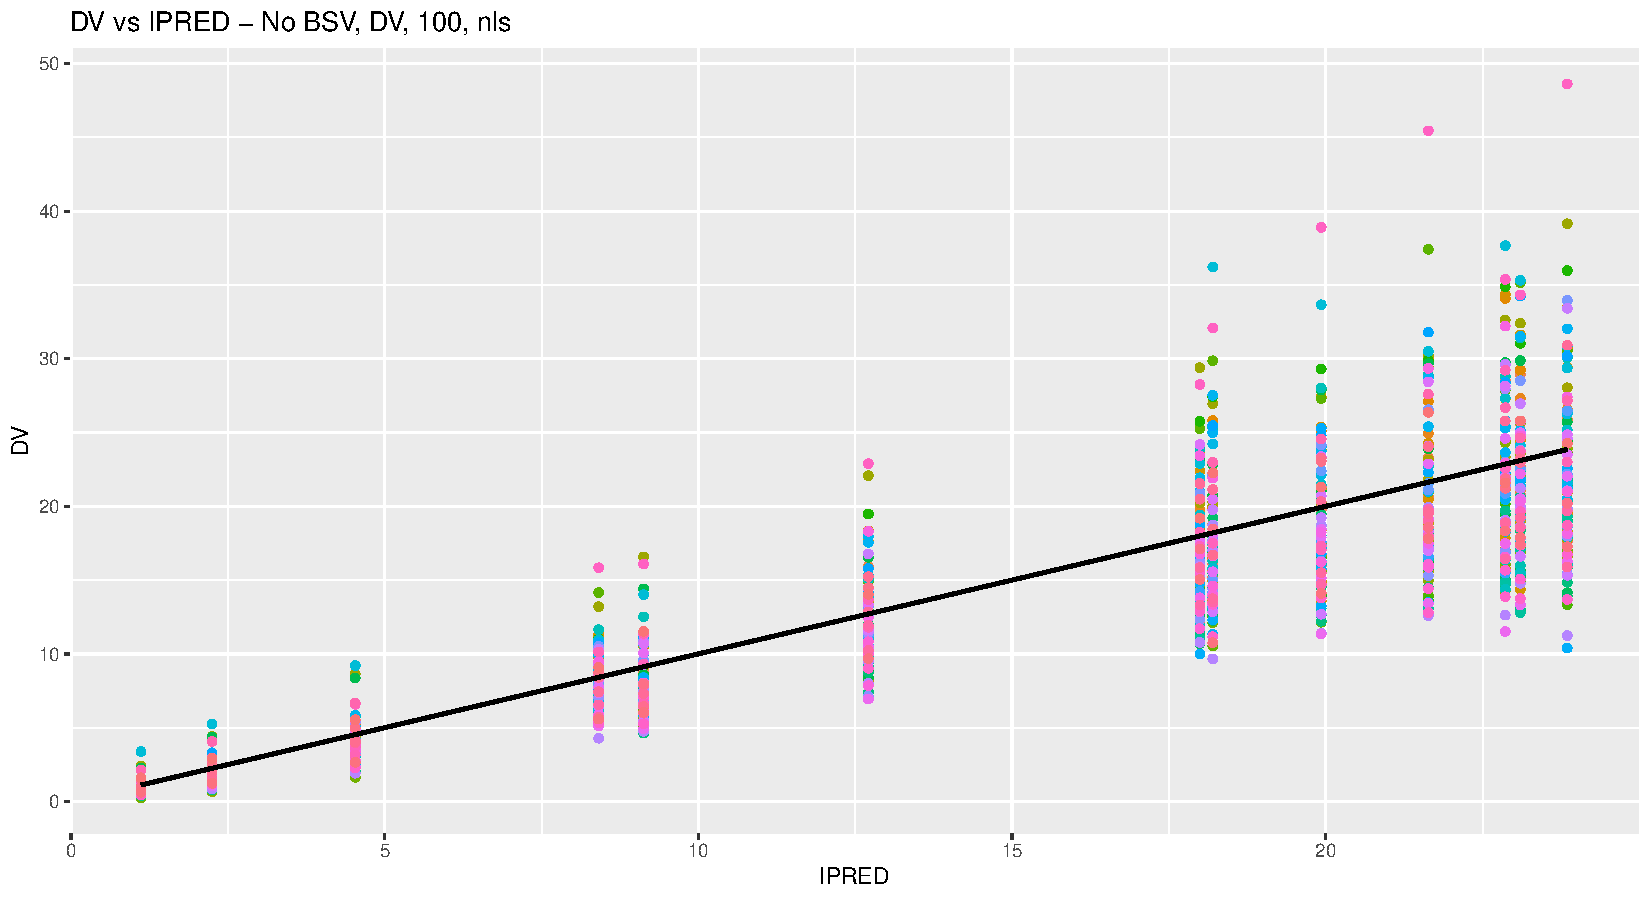
\includegraphics[width=\linewidth]{fig/img/Xpose/nobsv/dv_vs_ipred_100_nls_plot.pdf}
        \caption{}
        \label{fig:}
    \end{subfigure}
    
    \vspace{1em} % Adjust vertical space between rows

    \begin{subfigure}[b]{0.49\linewidth}
        \centering
        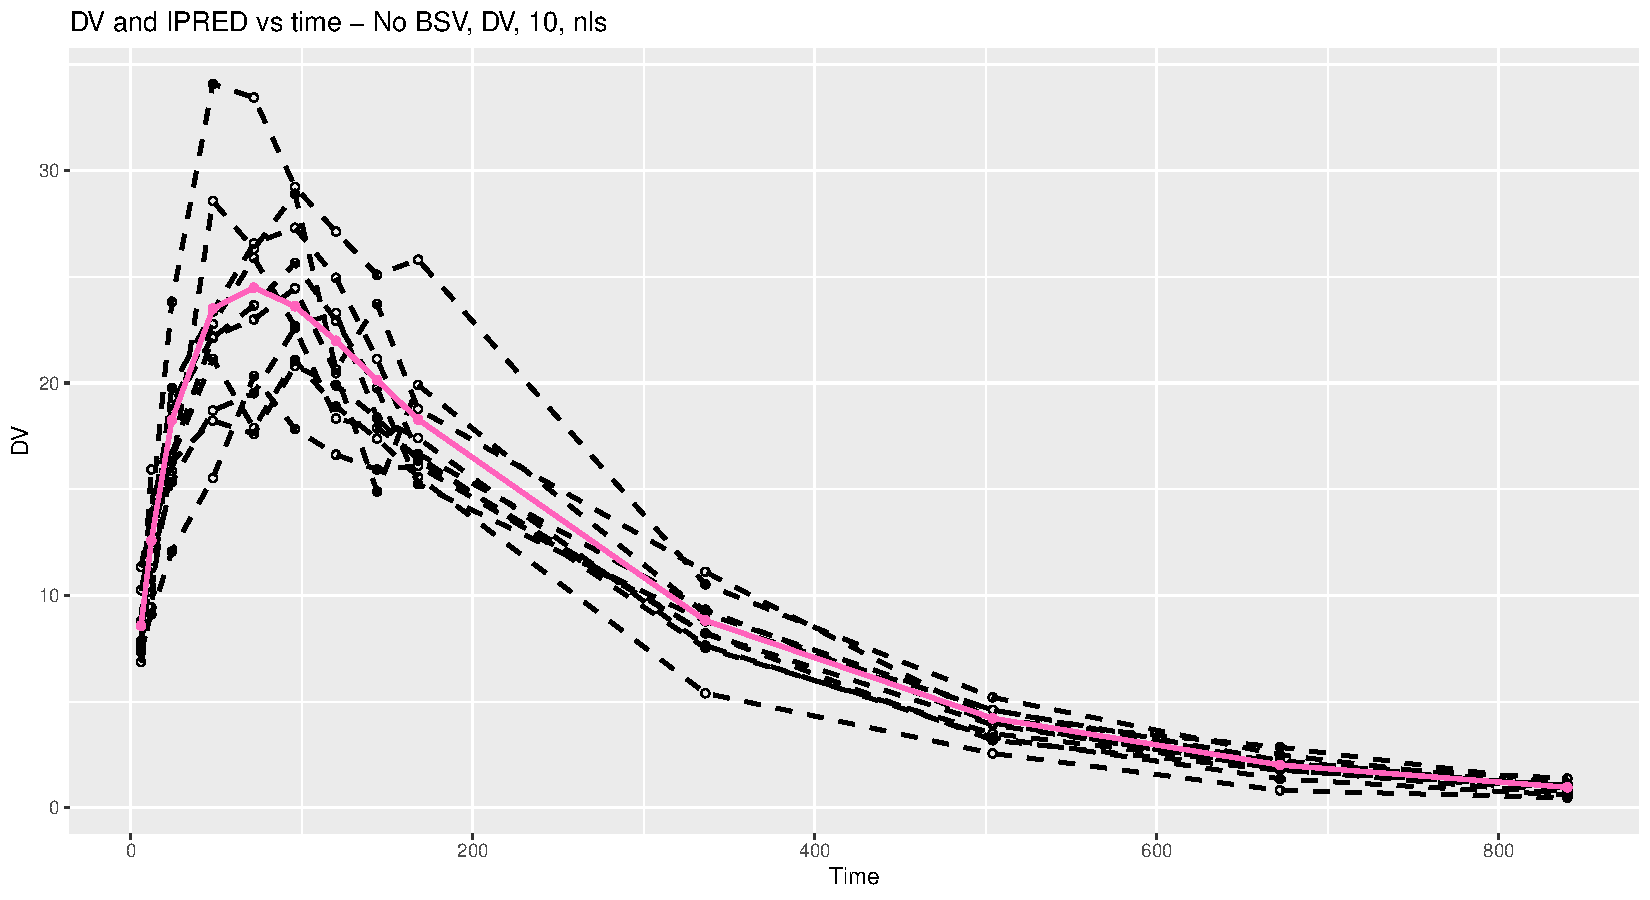
\includegraphics[width=\linewidth]{fig/img/Xpose/nobsv/dv_and_ipred_vs_time_10_nls_plot.pdf}
        \caption{}
        \label{fig:}
    \end{subfigure}
    \hfill
    \begin{subfigure}[b]{0.49\linewidth}
        \centering
        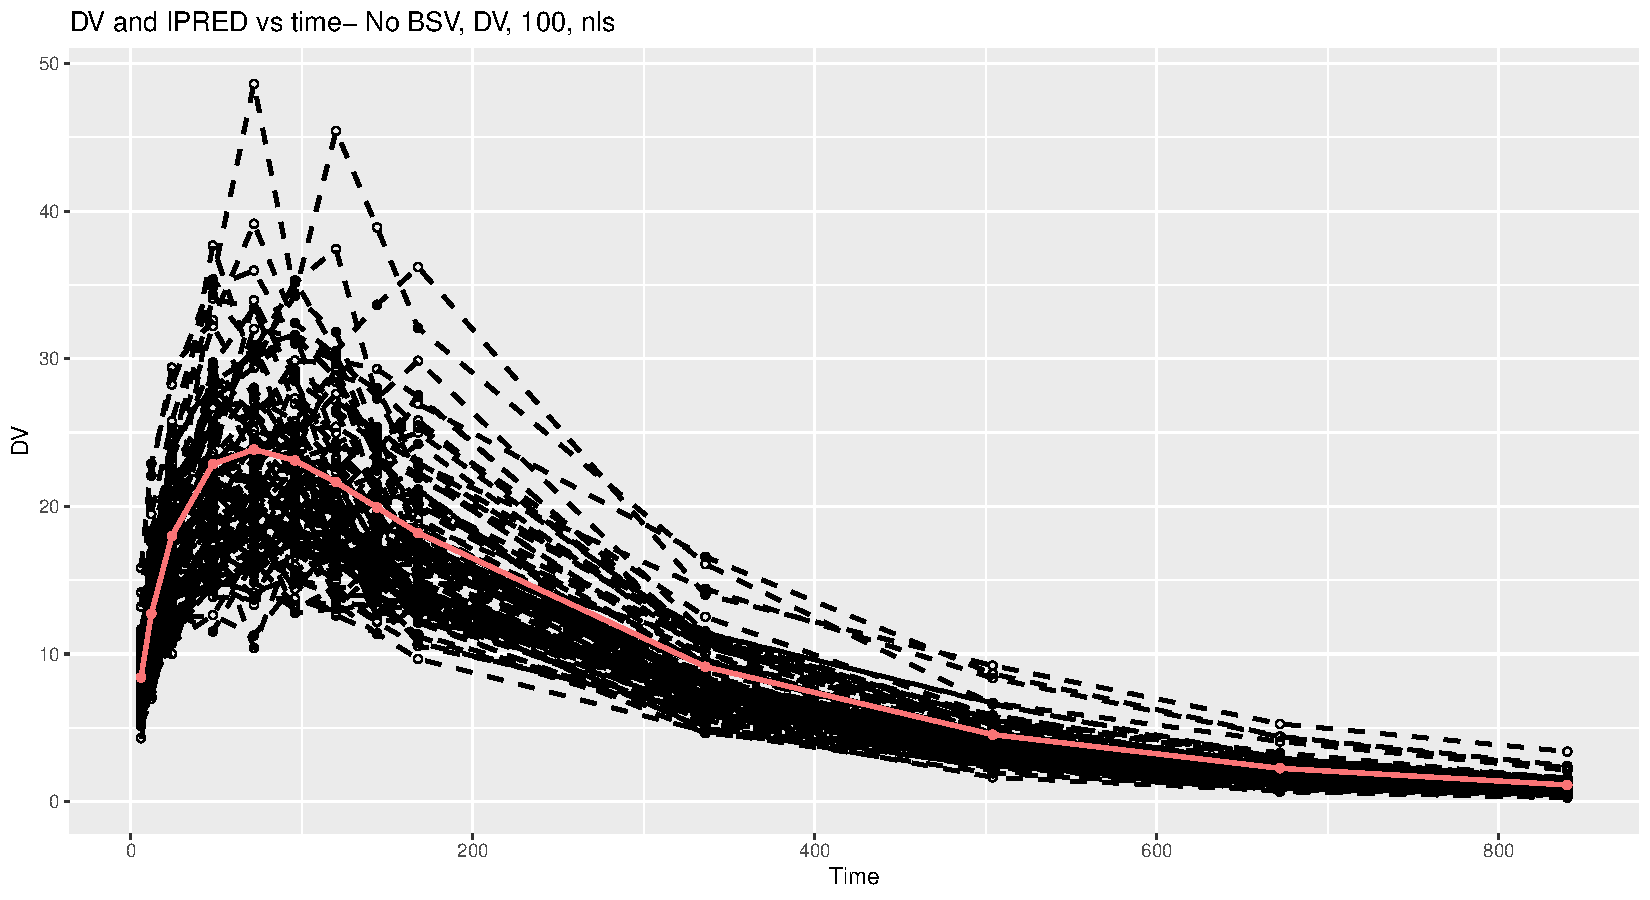
\includegraphics[width=\linewidth]{fig/img/Xpose/nobsv/dv_and_ipred_vs_time_100_nls_plot.pdf}
        \caption{}
        \label{fig:}
    \end{subfigure}
\end{figure}

\section{Model with ETAs on CL and Q}
A model is fitted with $\theta_i = (k_{a,\mu}, CL_{\mu}\cdot \ep{\eta_{CL,i}}, Q_{\mu}\cdot \ep{\eta_{CL,i}},V_{c,\mu},V_{p,\mu})^\top$.

\subsection{10 sample profile}
\begin{table}
\centering\centering
\caption{ETA CLQ DV 10}
\centering
\fontsize{8}{10}\selectfont
\begin{tabular}[t]{lllllll}
\toprule
\textbf{Parameter} & \textbf{Est} & \textbf{SE} & \textbf{\%RSE} & \textbf{Back-transformed} & \textbf{BSV} & \textbf{Shrinkage}\\
\midrule
tka & -3.56 & 0.0155 & 0.435 & 0.0284 (0.0275, 0.0292) &  & \\
\midrule
tq & -0.93 & 0.115 & 12.4 & 0.394 (0.315, 0.495) &  & \\
\midrule
tcl & -3.41 & 0.0434 & 1.27 & 0.0332 (0.0305, 0.0361) &  & \\
\midrule
tvc & 1.23 & 0.0909 & 7.37 & 3.44 (2.87, 4.11) &  & \\
\midrule
tvp & 1.31 & 0.0164 & 1.25 & 3.72 (3.6, 3.84) &  & \\
\midrule
prop.sd & 0.155 &  &  & 0.155 &  & \\
\midrule\\
eta.q &  &  &  &  & 9.15 & -0.392\%>\\
\bottomrule
\end{tabular}
\end{table}
\subsection{25 sample profile}
\begin{table}
\centering\centering
\caption{ETA CLQ DV 25}
\centering
\fontsize{8}{10}\selectfont
\begin{tabular}[t]{lllllll}
\toprule
\textbf{Parameter} & \textbf{Est} & \textbf{SE} & \textbf{\%RSE} & \textbf{Back-transformed} & \textbf{BSV} & \textbf{Shrinkage}\\
\midrule
tka & -3.62 & 0.519 & 14.3 & 0.0267 (0.00965, 0.0737) &  & \\
\midrule
tq & -1 & 1.5 & 149 & 0.366 (0.0193, 6.95) &  & \\
\midrule
tcl & -3.39 & 0.0485 & 1.43 & 0.0338 (0.0308, 0.0372) &  & \\
\midrule
tvc & 1.11 & 0.126 & 11.4 & 3.03 (2.36, 3.87) &  & \\
\midrule
tvp & 1.42 & 0.0319 & 2.25 & 4.15 (3.89, 4.41) &  & \\
\midrule
prop.sd & 0.183 &  &  & 0.183 &  & \\
\midrule\\
eta.q &  &  &  &  & 15.8 & 13.0\%<\\
\bottomrule
\end{tabular}
\end{table}
\subsection{50 sample profile}
\begin{table}
\centering\centering
\caption{ETA CLQ DV 50}
\centering
\fontsize{8}{10}\selectfont
\begin{tabular}[t]{lllllll}
\toprule
\textbf{Parameter} & \textbf{Est} & \textbf{SE} & \textbf{\%RSE} & \textbf{Back-transformed} & \textbf{BSV} & \textbf{Shrinkage}\\
\midrule
tka & -3.81 & 0.288 & 7.56 & 0.0223 (0.0127, 0.0391) &  & \\
\midrule
tq & -1.36 & 0.654 & 48.1 & 0.257 (0.0712, 0.924) &  & \\
\midrule
tcl & -3.34 & 0.0651 & 1.95 & 0.0354 (0.0311, 0.0402) &  & \\
\midrule
tvc & 1.08 & 0.261 & 24.3 & 2.94 (1.76, 4.9) &  & \\
\midrule
tvp & 1.49 & 0.124 & 8.34 & 4.42 (3.47, 5.64) &  & \\
\midrule
prop.sd & 0.211 &  &  & 0.211 &  & \\
\midrule\\
eta.q &  &  &  &  & 15.5 & 5.20\%<\\
\bottomrule
\end{tabular}
\end{table}
\subsection{100 sample profile}
\begin{table}
\centering\centering
\caption{ETA CLQ DV 100}
\centering
\fontsize{8}{10}\selectfont
\begin{tabular}[t]{lllllll}
\toprule
\textbf{Parameter} & \textbf{Est} & \textbf{SE} & \textbf{\%RSE} & \textbf{Back-transformed} & \textbf{BSV} & \textbf{Shrinkage}\\
\midrule
tka & -5.43 & 0.00643 & 0.118 & 0.00437 (0.00432, 0.00443) &  & \\
\midrule
tq & -2.12 & 0.0368 & 1.74 & 0.12 (0.112, 0.129) &  & \\
\midrule
tcl & -3.34 & 0.015 & 0.45 & 0.0353 (0.0343, 0.0364) &  & \\
\midrule
tvc & -1.15 & 0.041 & 3.57 & 0.317 (0.293, 0.344) &  & \\
\midrule
tvp & -0.349 & 0.0249 & 7.15 & 0.705 (0.672, 0.741) &  & \\
\midrule
prop.sd & 0.162 &  &  & 0.162 &  & \\
\midrule\\
eta.q &  &  &  &  & 25.2 & -0.192\%>\\
\bottomrule
\end{tabular}
\end{table}

\section{Model with ETAs on V2 and V3}
A model is fitted with $\theta_i = (k_{a,\mu}, CL_{\mu}, Q_{\mu},V_{c,\mu}\cdot \ep{\eta_{V,i}},V_{p,\mu}\cdot \ep{\eta_{V,i}})^\top$.

\subsection{10 sample profile}
\begin{table}
\centering\centering
\caption{ETA V DV 10}
\centering
\fontsize{8}{10}\selectfont
\begin{tabular}[t]{lllllll}
\toprule
\textbf{Parameter} & \textbf{Est} & \textbf{SE} & \textbf{\%RSE} & \textbf{Back-transformed} & \textbf{BSV} & \textbf{Shrinkage}\\
\midrule
tka & -3.67 & 1.4 & 38.2 & 0.0256 (0.00165, 0.398) &  & \\
\midrule
tq & -1.2 & 3.24 & 271 & 0.302 (0.000526, 174) &  & \\
\midrule
tcl & -3.42 & 0.105 & 3.07 & 0.0329 (0.0268, 0.0404) &  & \\
\midrule
tvc & 1.2 & 1.3 & 108 & 3.32 (0.261, 42.3) &  & \\
\midrule
tvp & 1.3 & 0.636 & 49.1 & 3.65 (1.05, 12.7) &  & \\
\midrule
prop.sd & 0.18 &  &  & 0.18 &  & \\
\midrule\\
eta.vp &  &  &  &  & 8.73 & 5.81\%<\\
\bottomrule
\end{tabular}
\end{table}
\subsection{25 sample profile}
\begin{table}
\centering\centering
\caption{ETA V DV 25}
\centering
\fontsize{8}{10}\selectfont
\begin{tabular}[t]{lllllll}
\toprule
\textbf{Parameter} & \textbf{Est} & \textbf{SE} & \textbf{\%RSE} & \textbf{Back-transformed} & \textbf{BSV} & \textbf{Shrinkage}\\
\midrule
tka & -3.65 & 0.0574 & 1.57 & 0.026 (0.0232, 0.0291) &  & \\
\midrule
tq & -1.29 & 0.287 & 22.2 & 0.275 (0.157, 0.482) &  & \\
\midrule
tcl & -3.4 & 0.0609 & 1.79 & 0.0335 (0.0297, 0.0378) &  & \\
\midrule
tvc & 1.21 & 0.0521 & 4.32 & 3.34 (3.01, 3.7) &  & \\
\midrule
tvp & 1.34 & 0.083 & 6.19 & 3.83 (3.25, 4.5) &  & \\
\midrule
prop.sd & 0.255 &  &  & 0.255 &  & \\
\midrule\\
eta.vp &  &  &  &  & 9.40 & 22.4\%=\\
\bottomrule
\end{tabular}
\end{table}
\subsection{50 sample profile}
\begin{table}
\centering\centering
\caption{ETA V DV 50}
\centering
\fontsize{8}{10}\selectfont
\begin{tabular}[t]{lllllll}
\toprule
\textbf{Parameter} & \textbf{Est} & \textbf{SE} & \textbf{\%RSE} & \textbf{Back-transformed} & \textbf{BSV} & \textbf{Shrinkage}\\
\midrule
tka & -3.54 & 0.119 & 3.36 & 0.0289 (0.0229, 0.0365) &  & \\
\midrule
tq & -0.505 & 0.318 & 63 & 0.604 (0.324, 1.13) &  & \\
\midrule
tcl & -3.36 & 0.0355 & 1.06 & 0.0349 (0.0326, 0.0374) &  & \\
\midrule
tvc & 1.19 & 0.0964 & 8.13 & 3.27 (2.71, 3.95) &  & \\
\midrule
tvp & 1.49 & 0.0497 & 3.32 & 4.45 (4.04, 4.91) &  & \\
\midrule
prop.sd & 0.286 &  &  & 0.286 &  & \\
\midrule\\
eta.vp &  &  &  &  & 11.3 & 28.3\%=\\
\bottomrule
\end{tabular}
\end{table}
\subsection{100 sample profile}
\begin{table}
\centering\centering
\caption{ETA V DV 100}
\centering
\fontsize{8}{10}\selectfont
\begin{tabular}[t]{lllllll}
\toprule
\textbf{Parameter} & \textbf{Est} & \textbf{SE} & \textbf{\%RSE} & \textbf{Back-transformed} & \textbf{BSV} & \textbf{Shrinkage}\\
\midrule
tka & -3.69 & 0.193 & 5.23 & 0.025 (0.0172, 0.0365) &  & \\
\midrule
tq & -1.04 & 0.635 & 61.2 & 0.354 (0.102, 1.23) &  & \\
\midrule
tcl & -3.38 & 0.0129 & 0.382 & 0.034 (0.0332, 0.0349) &  & \\
\midrule
tvc & 1.16 & 0.208 & 17.9 & 3.2 (2.13, 4.81) &  & \\
\midrule
tvp & 1.45 & 0.146 & 10.1 & 4.27 (3.21, 5.68) &  & \\
\midrule
prop.sd & 0.288 &  &  & 0.288 &  & \\
\midrule\\
eta.vp &  &  &  &  & 10.2 & 31.6\%>\\
\bottomrule
\end{tabular}
\end{table}

\section{Model with ETAs on all}
A model is fitted with $\theta_i = (k_{a,\mu}, CL_{\mu}\cdot \ep{\eta_{CL,i}}, Q_{\mu}\cdot \ep{\eta_{CL,i}},V_{c,\mu}\cdot \ep{\eta_{V,i}},V_{p,\mu}\cdot \ep{\eta_{V,i}})^\top$.

\subsection{10 sample profile}
\input{code/Data/Dataframes/parFixed_ETA_All_DV_10_Init_1}
\subsection{25 sample profile}
\input{code/Data/Dataframes/parFixed_ETA_All_DV_25_Init_1}
\subsection{50 sample profile}
\input{code/Data/Dataframes/parFixed_ETA_All_DV_50_Init_1}
\subsection{100 sample profile}
\input{code/Data/Dataframes/parFixed_ETA_All_DV_100_Init_1}

\section{Model with BW as covariate and ETAs on CL and Q}
A model is fitted with $$\theta_i = (k_{a,\mu}, CL_{\mu}\cdot \left(\frac{BW_i}{85}\right)^\alpha \cdot \ep{\eta_{CL,i}}, Q_{\mu}\cdot \left(\frac{BW_i}{85}\right)^\alpha \cdot\ep{\eta_{CL,i}},V_{c,\mu},V_{p,\mu})^\top$$.
\subsection{10 sample profile}
\begin{table}
\centering\centering
\caption{ETA CLQ DV 10}
\centering
\fontsize{8}{10}\selectfont
\begin{tabular}[t]{lllllll}
\toprule
\textbf{Parameter} & \textbf{Est} & \textbf{SE} & \textbf{\%RSE} & \textbf{Back-transformed} & \textbf{BSV} & \textbf{Shrinkage}\\
\midrule
tka & -3.58 & 1.01 & 28.3 & 0.0279 (0.00383, 0.203) &  & \\
\midrule
tq & -1.01 & 3.4 & 336 & 0.363 (0.000462, 286) &  & \\
\midrule
tcl & -3.36 & 0.103 & 3.05 & 0.0346 (0.0283, 0.0423) &  & \\
\midrule
tvc & 1.25 & 0.826 & 65.9 & 3.5 (0.694, 17.7) &  & \\
\midrule
tvp & 1.29 & 0.584 & 45.3 & 3.63 (1.16, 11.4) &  & \\
\midrule
pow1 & 0.401 & 0.58 & 145 & 0.401 (-0.736, 1.54) &  & \\
\midrule
prop.sd & 0.154 &  &  & 0.154 &  & \\
\midrule\\
eta.q &  &  &  &  & 7.87 & 4.49\%<\\
\bottomrule
\end{tabular}
\end{table}
\subsection{25 sample profile}
\begin{table}
\centering\centering
\caption{ETA CLQ DV 25}
\centering
\fontsize{8}{10}\selectfont
\begin{tabular}[t]{lllllll}
\toprule
\textbf{Parameter} & \textbf{Est} & \textbf{SE} & \textbf{\%RSE} & \textbf{Back-transformed} & \textbf{BSV} & \textbf{Shrinkage}\\
\midrule
tka & -3.57 & 0.108 & 3.03 & 0.0282 (0.0228, 0.0348) &  & \\
\midrule
tq & -0.633 & 0.468 & 73.8 & 0.531 (0.212, 1.33) &  & \\
\midrule
tcl & -3.36 & 0.0244 & 0.725 & 0.0347 (0.0331, 0.0364) &  & \\
\midrule
tvc & 1.02 & 0.0513 & 5.01 & 2.78 (2.52, 3.08) &  & \\
\midrule
tvp & 1.49 & 0.0397 & 2.66 & 4.46 (4.12, 4.82) &  & \\
\midrule
pow1 & 0.53 & 0.125 & 23.6 & 0.53 (0.284, 0.776) &  & \\
\midrule
prop.sd & 0.183 &  &  & 0.183 &  & \\
\midrule\\
eta.q &  &  &  &  & 9.09 & 4.42\%<\\
\bottomrule
\end{tabular}
\end{table}
\subsection{50 sample profile}
\begin{table}
\centering\centering
\caption{ETA CLQ DV 50}
\centering
\fontsize{8}{10}\selectfont
\begin{tabular}[t]{lllllll}
\toprule
\textbf{Parameter} & \textbf{Est} & \textbf{SE} & \textbf{\%RSE} & \textbf{Back-transformed} & \textbf{BSV} & \textbf{Shrinkage}\\
\midrule
tka & -3.73 & 0.334 & 8.97 & 0.024 (0.0125, 0.0463) &  & \\
\midrule
tq & -1.02 & 0.868 & 85.3 & 0.361 (0.0659, 1.98) &  & \\
\midrule
tcl & -3.34 & 0.0463 & 1.39 & 0.0353 (0.0322, 0.0387) &  & \\
\midrule
tvc & 1.05 & 0.305 & 29.2 & 2.85 (1.56, 5.18) &  & \\
\midrule
tvp & 1.54 & 0.166 & 10.8 & 4.66 (3.36, 6.45) &  & \\
\midrule
pow1 & 0.56 & 0.269 & 48 & 0.56 (0.0331, 1.09) &  & \\
\midrule
prop.sd & 0.211 &  &  & 0.211 &  & \\
\midrule\\
eta.q &  &  &  &  & 11.9 & 11.2\%<\\
\bottomrule
\end{tabular}
\end{table}
\subsection{100 sample profile}
\begin{table}
\centering\centering
\caption{ETA CLQ DV 100}
\centering
\fontsize{8}{10}\selectfont
\begin{tabular}[t]{lllllll}
\toprule
\textbf{Parameter} & \textbf{Est} & \textbf{SE} & \textbf{\%RSE} & \textbf{Back-transformed} & \textbf{BSV} & \textbf{Shrinkage}\\
\midrule
tka & -3.69 & 0.146 & 3.97 & 0.025 (0.0188, 0.0333) &  & \\
\midrule
tq & -1.01 & 0.456 & 45.1 & 0.364 (0.149, 0.89) &  & \\
\midrule
tcl & -3.36 & 0.0286 & 0.852 & 0.0348 (0.0329, 0.0368) &  & \\
\midrule
tvc & 1.1 & 0.133 & 12.2 & 3 (2.31, 3.89) &  & \\
\midrule
tvp & 1.5 & 0.0852 & 5.69 & 4.46 (3.78, 5.27) &  & \\
\midrule
pow1 & 0.61 & 0.156 & 25.6 & 0.61 (0.304, 0.915) &  & \\
\midrule
prop.sd & 0.207 &  &  & 0.207 &  & \\
\midrule\\
eta.q &  &  &  &  & 11.4 & 5.29\%<\\
\bottomrule
\end{tabular}
\end{table}

\section{Model with BW as covariate and ETAs on V2 and V3}
\subsection{10 sample profile}
\begin{table}
\centering\centering
\caption{ETA V DV 10}
\centering
\fontsize{8}{10}\selectfont
\begin{tabular}[t]{lllllll}
\toprule
\textbf{Parameter} & \textbf{Est} & \textbf{SE} & \textbf{\%RSE} & \textbf{Back-transformed} & \textbf{BSV} & \textbf{Shrinkage}\\
\midrule
tka & -3.53 & 1.46 & 41.3 & 0.0294 (0.00169, 0.512) &  & \\
\midrule
tq & -0.758 & 4.79 & 632 & 0.468 (3.89e-05, 5.63e+03) &  & \\
\midrule
tcl & -3.41 & 0.0975 & 2.86 & 0.033 (0.0272, 0.0399) &  & \\
\midrule
tvc & 1.34 & 1.13 & 84.9 & 3.81 (0.412, 35.2) &  & \\
\midrule
tvp & 1.4 & 0.917 & 65.4 & 4.07 (0.674, 24.5) &  & \\
\midrule
pow1 & 0.764 & 1.15 & 151 & 0.764 (-1.49, 3.02) &  & \\
\midrule
prop.sd & 0.179 &  &  & 0.179 &  & \\
\midrule\\
eta.vp &  &  &  &  & 18.1 & 15.0\%<\\
\bottomrule
\end{tabular}
\end{table}
\subsection{25 sample profile}
\begin{table}
\centering\centering
\caption{ETA V DV 25}
\centering
\fontsize{8}{10}\selectfont
\begin{tabular}[t]{lllllll}
\toprule
\textbf{Parameter} & \textbf{Est} & \textbf{SE} & \textbf{\%RSE} & \textbf{Back-transformed} & \textbf{BSV} & \textbf{Shrinkage}\\
\midrule
tka & -3.59 & 0.875 & 24.4 & 0.0276 (0.00496, 0.153) &  & \\
\midrule
tq & -0.762 & 2.36 & 310 & 0.467 (0.00456, 47.8) &  & \\
\midrule
tcl & -3.39 & 0.0566 & 1.67 & 0.0337 (0.0302, 0.0377) &  & \\
\midrule
tvc & 1.05 & 0.843 & 80.4 & 2.85 (0.546, 14.9) &  & \\
\midrule
tvp & 1.45 & 0.511 & 35.2 & 4.27 (1.57, 11.6) &  & \\
\midrule
pow1 & -0.241 & 0.218 & 90.2 & -0.241 (-0.668, 0.185) &  & \\
\midrule
prop.sd & 0.258 &  &  & 0.258 &  & \\
\midrule\\
eta.vp &  &  &  &  & 7.34 & 21.7\%=\\
\bottomrule
\end{tabular}
\end{table}
\subsection{50 sample profile}
\begin{table}
\centering\centering
\caption{ETA V DV 50}
\centering
\fontsize{8}{10}\selectfont
\begin{tabular}[t]{lllllll}
\toprule
\textbf{Parameter} & \textbf{Est} & \textbf{SE} & \textbf{\%RSE} & \textbf{Back-transformed} & \textbf{BSV} & \textbf{Shrinkage}\\
\midrule
tka & -3.71 & 0.0241 & 0.649 & 0.0244 (0.0233, 0.0256) &  & \\
\midrule
tq & -1.22 & 0.0656 & 5.37 & 0.295 (0.259, 0.335) &  & \\
\midrule
tcl & -3.36 & 0.0392 & 1.17 & 0.0349 (0.0323, 0.0377) &  & \\
\midrule
tvc & 1.21 & 0.0475 & 3.93 & 3.35 (3.05, 3.68) &  & \\
\midrule
tvp & 1.43 & 0.0292 & 2.05 & 4.17 (3.94, 4.41) &  & \\
\midrule
pow1 & 0.0364 & 0.0992 & 272 & 0.0364 (-0.158, 0.231) &  & \\
\midrule
prop.sd & 0.282 &  &  & 0.282 &  & \\
\midrule\\
eta.vp &  &  &  &  & 13.7 & 27.5\%=\\
\bottomrule
\end{tabular}
\end{table}
\subsection{100 sample profile}
\begin{table}
\centering\centering
\caption{ETA V DV 100}
\centering
\fontsize{8}{10}\selectfont
\begin{tabular}[t]{lllllll}
\toprule
\textbf{Parameter} & \textbf{Est} & \textbf{SE} & \textbf{\%RSE} & \textbf{Back-transformed} & \textbf{BSV} & \textbf{Shrinkage}\\
\midrule
tka & -3.69 & 0.163 & 4.41 & 0.025 (0.0182, 0.0344) &  & \\
\midrule
tq & -1.29 & 0.425 & 33 & 0.276 (0.12, 0.635) &  & \\
\midrule
tcl & -3.38 & 0.012 & 0.355 & 0.034 (0.0332, 0.0348) &  & \\
\midrule
tvc & 1.28 & 0.202 & 15.7 & 3.61 (2.43, 5.36) &  & \\
\midrule
tvp & 1.41 & 0.16 & 11.3 & 4.1 (3, 5.61) &  & \\
\midrule
pow1 & 0.384 & 0.243 & 63.2 & 0.384 (-0.0914, 0.859) &  & \\
\midrule
prop.sd & 0.29 &  &  & 0.29 &  & \\
\midrule\\
eta.vp &  &  &  &  & 15.4 & 26.9\%=\\
\bottomrule
\end{tabular}
\end{table}

\section{Model with BW as covariate and ETAs on all}
\subsection{10 sample profile}
\input{code/Data/Dataframes/BW.parFixed_BW_ETA_All_DV_10_Init_1}
\subsection{25 sample profile}
\input{code/Data/Dataframes/BW.parFixed_BW_ETA_All_DV_25_Init_1}
\subsection{50 sample profile}
\input{code/Data/Dataframes/BW.parFixed_BW_ETA_All_DV_50_Init_1}
\subsection{100 sample profile}
\input{code/Data/Dataframes/BW.parFixed_BW_ETA_All_DV_100_Init_1}